\documentclass[a4paper,12pt,oneside,openany]{book}	
\usepackage{layout}
\setlength{\textwidth}{15.0 cm}
\setlength{\textheight}{25.0 cm}


\usepackage[english,brazil]{babel}
\usepackage{pagina}	% pagina-padrao
\usepackage{indentfirst}		% for indent
\usepackage[latin1]{inputenc}
\usepackage{graphics,epsfig}
\usepackage{graphics}
\graphicspath{{./figuras/}}
\usepackage{pstricks,pst-node,pst-tree}
\usepackage{alltt}
%\usepackage{makeidx}
%\makeindex
\usepackage[figuresright]{rotating} % for saydways tables and figures
\usepackage{enumerate}			% for configuration of enumerate environment
\usepackage{amsmath}
\usepackage{amssymb}
\usepackage{multirow}

\setcounter{secnumdepth}{3}	% numeracao ate subsubsecao
\setcounter{tocdepth}{2}	% indice ate subsubsecao

\usepackage{longtable}


%Include Only --------
%Usar Include Only se quiser compilar apenas 1 capitulo.
%\includeonly{cap1}
%\includeonly{cap2}

\begin{document}

\frontmatter
\thispagestyle{empty}


\includegraphics[scale=0.7]{./FIGURAS/Poli.pdf}

\begin{center}
\large{Sistema de Direcionamento Autom�tico de Microfones para Eventos Esportivos.}\\
   \vspace{2cm}
\large{Felipe Ferreira da Silva}\\
\large{Jo�o Felipe Guedes da Silva}\\
\end{center}
   \vspace{3cm}
\hspace{7cm}
\hfill \parbox{8.0cm}{Relat�rio da disciplina Projeto Integrado do Curso de Engenharia 
Eletr�nica e de Computa��o da Escola Polit�cnica, Universidade Federal do Rio 
de Janeiro.\\}
   \vspace{2cm}
\hfill \parbox{8.0cm}{Professor: Carlos Jos� Ribas D'�vila} \\
\hfill \parbox{8.0cm}{Professor: Joarez Bastos Monteiro} \\
   \vspace{2cm}
\begin{center}
Rio de Janeiro

\today
\end{center}






\pagebreak            


% Siglas
\begin{center}
\textbf{SIGLAS}
\end{center}
      \vspace{0.5cm}

\paragraph{}UFRJ - Universidade Federal do Rio de Janeiro 


\pagebreak









% Table of Contents
% ---------------------------------------------------------------
     \tableofcontents
% ---------------------------------------------------------------
% Lista de figuras
% ---------------------------------------------------------------
%\cleardoublepage
%\addcontentsline{toc}{chapter}{Lista de Figuras}
\listoffigures
% ---------------------------------------------------------------
% Lista de Tabelas
% ---------------------------------------------------------------
%\cleardoublepage
%\addcontentsline{toc}{chapter}{Lista de Tabelas}
\listoftables

\mainmatter
\cleardoublepage
% ---------------------------------------------------------------
% Chapter 1 - Introdu��o
% ---------------------------------------------------------------
\chapter{Introdu��o}
\label{cap1}
% ---------------------------------------------------------------
% Chapter 1 - Introdu��o
% ---------------------------------------------------------------

\section{Motiva��o}

\section{Objetivo}

%\paragraph{}

	O presente trabalho tem como tem�tica...



%% ---------------------------------------------------------------
% Chapter 1 - Introdu��o
% ---------------------------------------------------------------

\section{Motiva��o}

\section{Objetivo}

%\paragraph{}

	O presente trabalho tem como tem�tica...




% ---------------------------------------------------------------
% Chapter 2 - Projeto
% ---------------------------------------------------------------
\chapter{Projeto}
\label{cap2}
% ---------------------------------------------------------------
% Chapter 2 - Projeto
% ---------------------------------------------------------------

\section{Caracteriza��o}
		
\section{Open CV}

	
%% ---------------------------------------------------------------
% Chapter 2 - Projeto
% ---------------------------------------------------------------

\section{Caracteriza��o}
		
\section{Open CV}

	

% ---------------------------------------------------------------
% Chapter 3 - Resultados
% ---------------------------------------------------------------
\chapter{Resultados}
\label{cap3}
% ---------------------------------------------------------------
% Chapter 3 - Resultados
% ---------------------------------------------------------------

\section{Imagens}

%% ---------------------------------------------------------------
% Chapter 2 - Projeto
% ---------------------------------------------------------------

\section{Caracteriza��o}
		
\section{Open CV}

	

%  ---------------------------------------------------------------
% Chapter 4 - Conclus�es
% ---------------------------------------------------------------
\chapter{Conclus�es}
\label{cap4}
%  ---------------------------------------------------------------
% Chapter 4 - Conclus�es
% ---------------------------------------------------------------

%%  ---------------------------------------------------------------
% Chapter 4 - Conclus�es
% ---------------------------------------------------------------


% ---------------------------------------------------------------
% Bibliografia
% ---------------------------------------------------------------
% \normalsize
% \cleardoublepage
% \addcontentsline{toc}{chapter}{Bibliografia}
% \bibliographystyle{coppe}
% \bibliography{biblio}

% ---------------------------------------------------------------
% Ap�ndices 
% ---------------------------------------------------------------
%   \appendix
   % ---------------------------------------------------------------
   % Ap�ndice A
   % ---------------------------------------------------------------
%   \chapter{O que � um ap�ndice}
%   \label{ApendiceA}
%   \paragraph{}Elemento que consiste em um texto ou documento elaborado pelo autor, com o intuito de complementar sua argumenta��o, sem preju�zo do trabalho. S�o identificados por letras mai�sculas consecutivas e pelos respectivos t�tulos.
   % ---------------------------------------------------------------
   % Ap�ndice B
   % ---------------------------------------------------------------
%   \chapter{Encaderna��o do Projeto de Gradua��o}
%   \label{ApendiceB}
%   \begin{figure}
	\begin{center}
		\parbox[htb]{13.0cm}
		{
		\begin{center}
			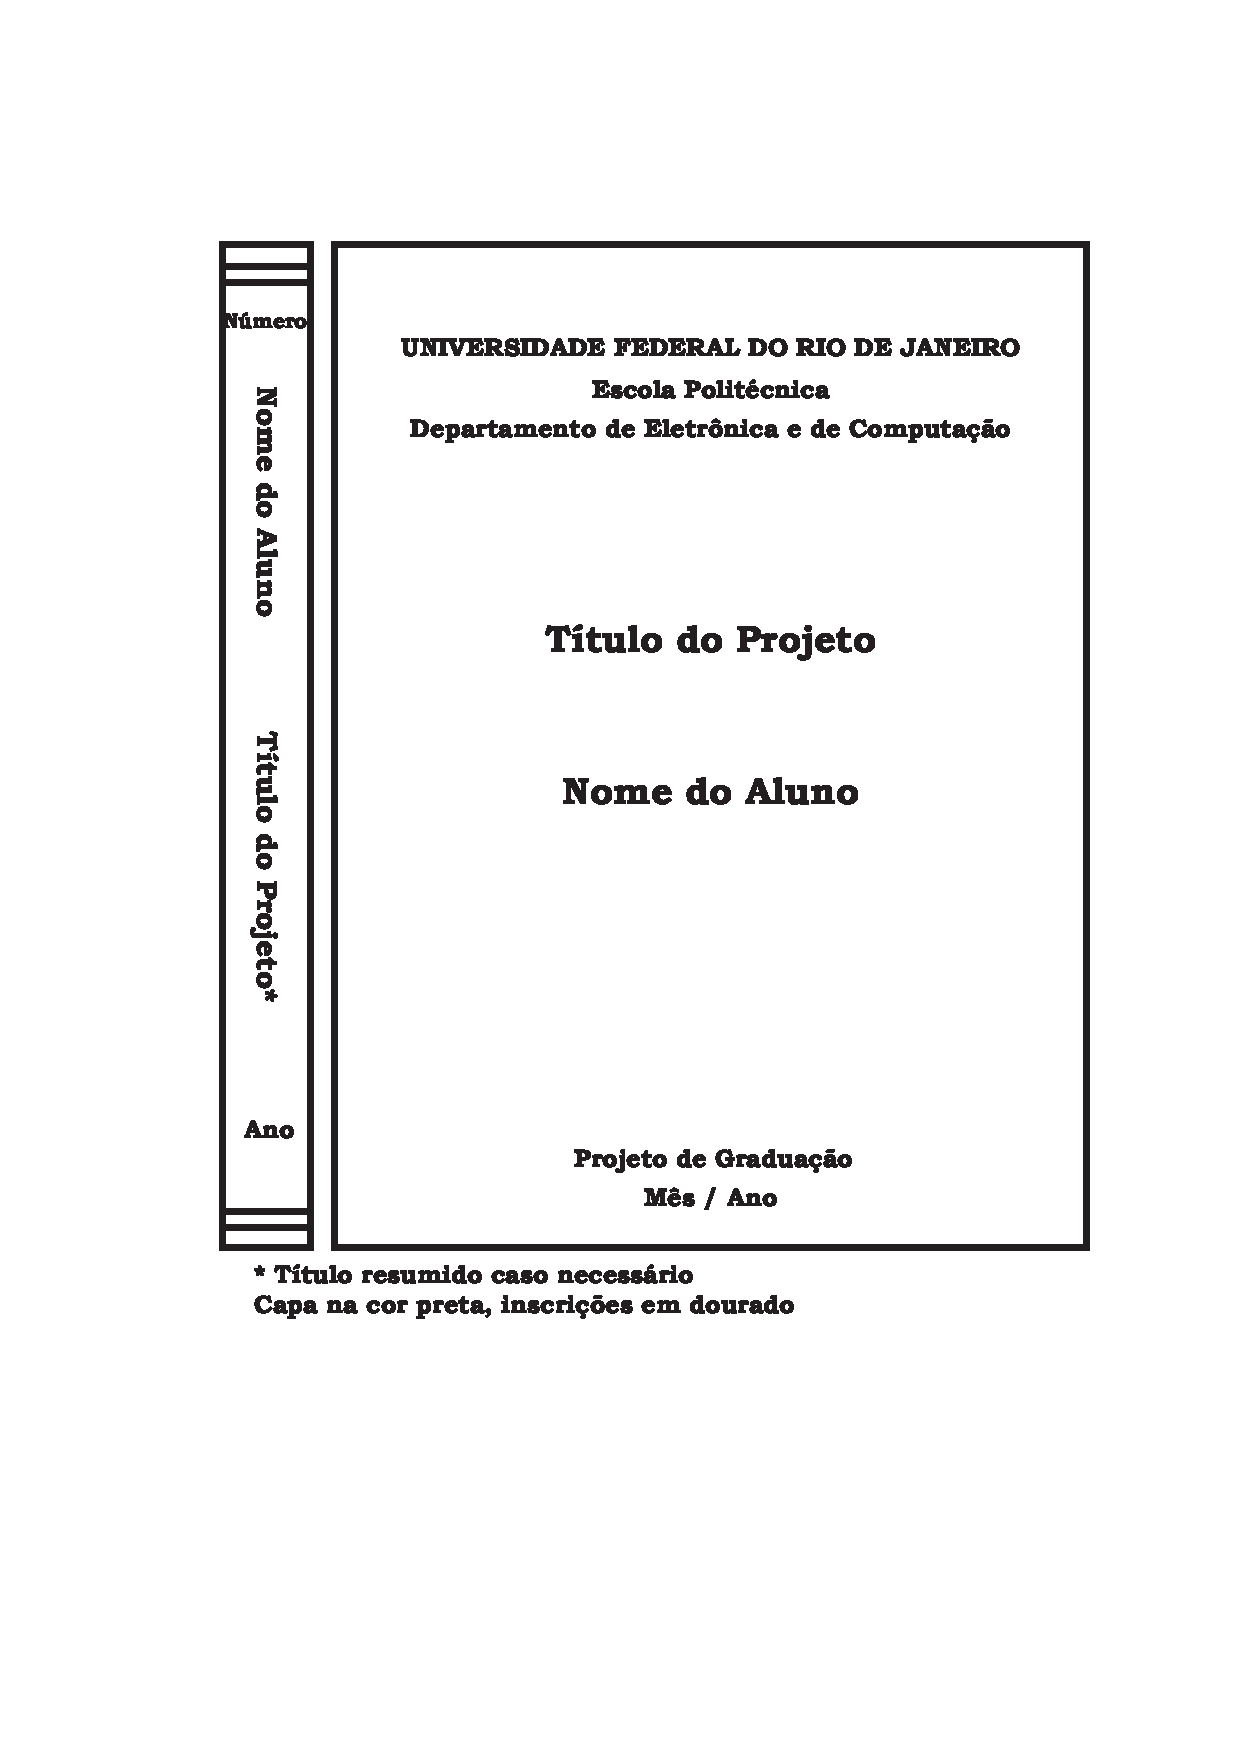
\includegraphics[scale=1.0]{Capa_do_Projeto_Final.pdf}
			\caption[\small{Encaderna��o do projeto de gradua��o.}]{\label{FigPFC} 
				\small{Encaderna��o do projeto de gradua��o.}}
		\end{center}
		}
	\end{center}
\end{figure}
   % ---------------------------------------------------------------
   % Ap�ndice C
   % ---------------------------------------------------------------
%   \chapter{O que � um anexo}
%   \label{ApendiceC}
%   \paragraph{}Documenta��o n�o elaborada pelo autor, ou elaborada pelo autor mas constituindo parte de outro projeto.   

\backmatter

\end{document}
